\subsection{Fourier transform of a synthetic signal}
The signal 
\begin{equation}
	s[t] = \sum_{k=0}^{10}\cos(2\pi\cdot2^k f_0\cdot t +k\cdot\frac{\pi}{3}) \quad f_0 = 100
\end{equation}
Can be generated with the following Matlab code
\begin{lstlisting}[
style=Matlab-editor,
basicstyle=\ttfamily\footnotesize,
numbers=none]
% Synthesizing the signal s[t]
T = 2; %period of 2s
N = 10; %sum limit
f0 = 100; %lowest frequency in generated signal
%Highest frequency is 2^N*f0=1024*100=1.024e5, choosing fs 4 times that
fs = 2^N*f0*10;
t = [0:1/fs:T-1/fs]; %time vector

% Generate signal
s = zeros(1,length(t));
for k = 0:N;
    s = s + cos(2*pi*2^k*f0*t+k*pi/3);
end
\end{lstlisting}
An excerpt of the generated signal can be seen in figure~\ref{fig:1.2-1}
\begin{figure}
	\center
	\includegraphics{./picture/3-1-2.eps}
	\caption{\(s[t]\) for \(0.9< t<0.93\)}
	\label{fig:1.2-1}
\end{figure}

The spectrum of \(s\) should contain peaks at \(2^kf_0\) for \(k=1\ldots 10\) with magnitude 1. As there is a phase difference 
between the individual sinusoids composing the signal, these peaks will be composed of differing real and imaginary parts. Looking
at the magnitude, real and imaginary spectrum in figure~\ref{fig:1.2-2} we see that this is true. 


\begin{figure}[H]
	\center
	\includegraphics{./picture/3-1-3.eps}
	\caption{Magnitude spectrum of \(s\) including the real and imaginary parts it is composed of. The real and imaginary parts 
	show a non-zero phase.}
	\label{fig:1.2-2}
\end{figure}

As the distance between peaks grows exponentially, it is quite hard to see what is going on around \(f=0Hz\), figure~\ref{fig:1.2-3}
therefore shows a dB-logarithmic plot of the magnitude spectrum of \(s\).

\begin{figure}[H]
	\center
	\includegraphics{./picture/3-1-4.eps}
	\caption{Magnitude spectrum of \(s\) showing dB on the y-axis and equally spaced peaks on the logarithmix frequency axis.
	The peak corresponding to the base frequency, \(f_0\) is marked in red.}
	\label{fig:1.2-3}
\end{figure}

Zooming in on the peak at \(f=400\)Hz, as done in figure~\ref{fig:1.2-4}, we see that it has a value of 1 as expected. However, 
it looks like the peak is actually a small triangle, but this is false. The triangle is a result of Matlab trying to plot a 
continuous curve. Since the signal has a period of 2 seconds, the resolution in the frequency domain is 0.5Hz. This means we
see the peak at 400Hz, while the closest defined values at 399.5Hz and 400.5Hz are 0. We do not have any information about the
frequencies between these points. A stem plot would better highlight this fact.

\begin{figure}[H]
	\center
	\includegraphics{./picture/3-1-5.eps}
	\caption{Zoom-in of the peak at 400Hz. This highlights Matlabs attempts to draw a continuous curve, even though we have no information about the points between \(f=399.5\)Hz and \(f=400.5\)Hz because of the 2s signal period.}
	\label{fig:1.2-3}
\end{figure}

We can write the signal to a wave file in order to check for distortion with the following matlab code. It is important to note
that wave files clip everything with a value above 1.0, so the signal must be scaled on write and read to avoid losing information.
\begin{lstlisting}[
style=Matlab-editor,
basicstyle=\ttfamily\footnotesize,
numbers=none]
% save s to ha3_s_12.wav
NBits = 16;
name = 'ha3_s_12.wav';
wavwrite(s/max(abs(s)),fs,NBits,name); %s has to be scaled to between -1 and 1 or it will be clipped
%read it back in
s_wav = wavread(name)'*max(abs(s)); %convert to row vector and scale to orignal
\end{lstlisting}

Figure~\ref{fig:1.2-4} shows the successful reconstruction of the signal in Matlab after having converted it to wave format. It
is clear that there is no distortion, which is expected since the wave file format is lossless.


\begin{figure}[H]
	\center
	\includegraphics{./picture/3-1-6.eps}
	\caption{Comparison between the original \(s\) signal and the reconstructed signal after conversion to wave format.}
	\label{fig:1.2-3}
\end{figure}
